\specialsection{Обзор литературы}

В последние годы отмечается значительный прогресс в области использования нейронных сетей для выявления мошенничества. Особый интерес исследователей вызывают графовые архитектуры, эффективно применяемые в различных прикладных задачах. Такая структура позволяет формализовать взаимосвязи между объектами, что делает их особенно подходящими для моделирования разнообразных мошеннических схем.

Одним из ключевых элементов современных графовых нейронных сетей является так называемый модуль обмена сообщениями, известный как Graph SAmple and aggreGatE (GraphSAGE) \cite{hamilton2017}. Этот подход обобщает концепцию сверточных нейронных сетей, применяемых в обработке изображений (Computer Vision, CV), на структуры графов, что позволяет учитывать информацию о соседних узлах. В работе сперва случайным образом выбираются и затем агрегируются векторы представлений вершин из окрестности данной, что улучшает ее признаковое описание, как бы собирая информацию о всем графе. Главным недостатком такого подхода является чрезмерное усреднение скрытых представлений, также часто называемых эмбедингами (embeddings), что ухудшает разделимость классов в силу их неразличимости.

Логичным продолжением развития графовых сверток стало внедрение механизма внимания \cite{vaswani2017}. Этот модуль получил название Graph ATtention network (GAT) \cite{velickovic2017} и, будучи заимствован из области обработки естественного языка (Natural Language Processing, NLP), сразу стал неотъемлемой частью практически всех архитектур обнаружения мошенничества. Он позволил моделировать неоднородные взаимосвязи между узлами графа, акцентируя внимание на наиболее важных вершинах из окрестности данной при вычислении ее представления.

Помимо GraphSAGE и GAT, исследователи создают и менее обобщенные в своем применении модули для нейронных сетей, например, Graph Convolutional Network (GCN) \cite{kipf2017}. Авторы данной свертки использовали графовый лапласиан для анализа процесса диффузии сигнала внутри него, показав отличное качество работы в задачах классификации вершин в графах цитирований и знаний. Однако, различные модификации этой концепции применяются и в других областях, например, для получения устойчивых векторных представлений узлов и для кластеризации вершин. В дальнейшем тексте будут рассмотрены и другие актуальные подходы, часто опирающиеся или напрямую включающие в себя принципы работы перечисленных моделуй.

CAmouflage-REsistant Graph Neural Network (CARE-GNN) \cite{dou2020} стала первой работой, в которой рассматривалась задача обнаружения мошенников на сайтах-агрегаторах отзывов Amazon и Yelp. Авторы обратили внимание на то, что злоумышленники часто маскируют свои намерения, взаимодействуя с разными классами пользователей. Такие графы называют гетерогенными, так как в них вершины из разных групп имеют общие ребра, то есть являются инцидентными. Для борьбы с проблемой усреднения признаков исследователи предложили использовать только часть узлов из окрестности вершины, как это делается в работе GraphSAGE. Процент выбранных узлов \(p\) является параметром, который находится с помощью многорукого бандита Бернулли из области обучения с подкреплением (Reinforcement Learning, RL). Схема полученной системы представлена на рис. \ref{dou2020_arch}.

\begin{figure}[ht]
\begin{center}
\scalebox{0.38}{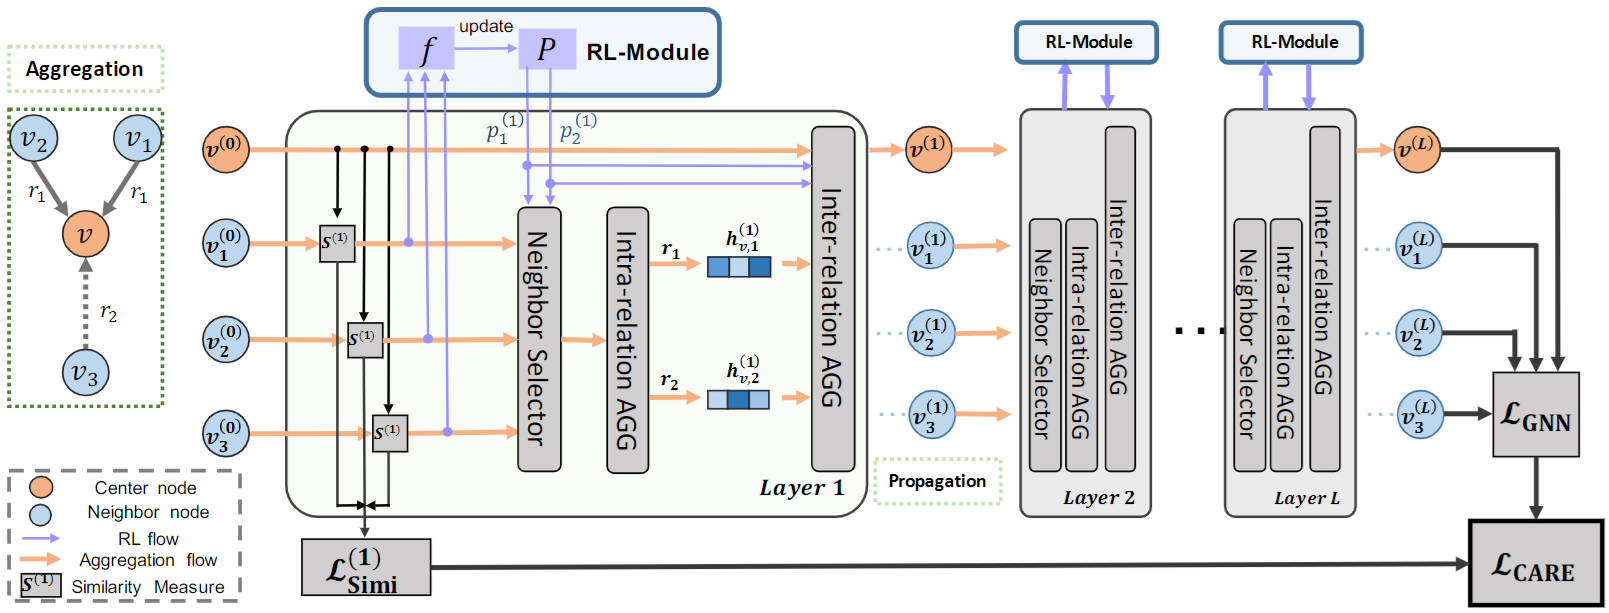
\includegraphics{images/dou2020_arch.png}}
\caption{\label{dou2020_arch} Архитектура CARE-GNN: из выбранных соседей узла \(v\) только \(p\) попадают на следующий слой, что позволяет распространять информацию по графу, не слишком усредняя представления каждой вершины.}
\end {center}
\end {figure}

Авторы работы Neural meta-Graph Search (NGS) \cite{qin2022} сосредоточились на объяснимости моделей и возможности обосновать полученные предсказания. Для этого исследователи сохраняют промежуточные состояния графа после применения сверток на каждом слое и используют их для предсказания на полученном метаграфе. Объяснимость особенно важна при использовании нейронных сетей в реальной жизни, так как невозможность разобрать полученное предсказание замедляет выявление ошибок модели.

Gated Temporal Attention Network (GTAN) \cite{xiang2023} и Group AGgregation enhanced trAnsformer (GAGA) \cite{wang2023} активно используют механизм внимания GAT для получения эмбедингов вершин и ребер. В частности, авторы GAGA много внимания уделяют проблеме гетерогенных графов, предварительно группируя узлы из окрестности по классам, что приводит к более выразительным представлениям в конце. Более подробно о составляющих GAGA можно посмотреть на рис. \ref{wang2023_arch}.

\begin{figure}[ht]
\begin{center}
\scalebox{0.46}{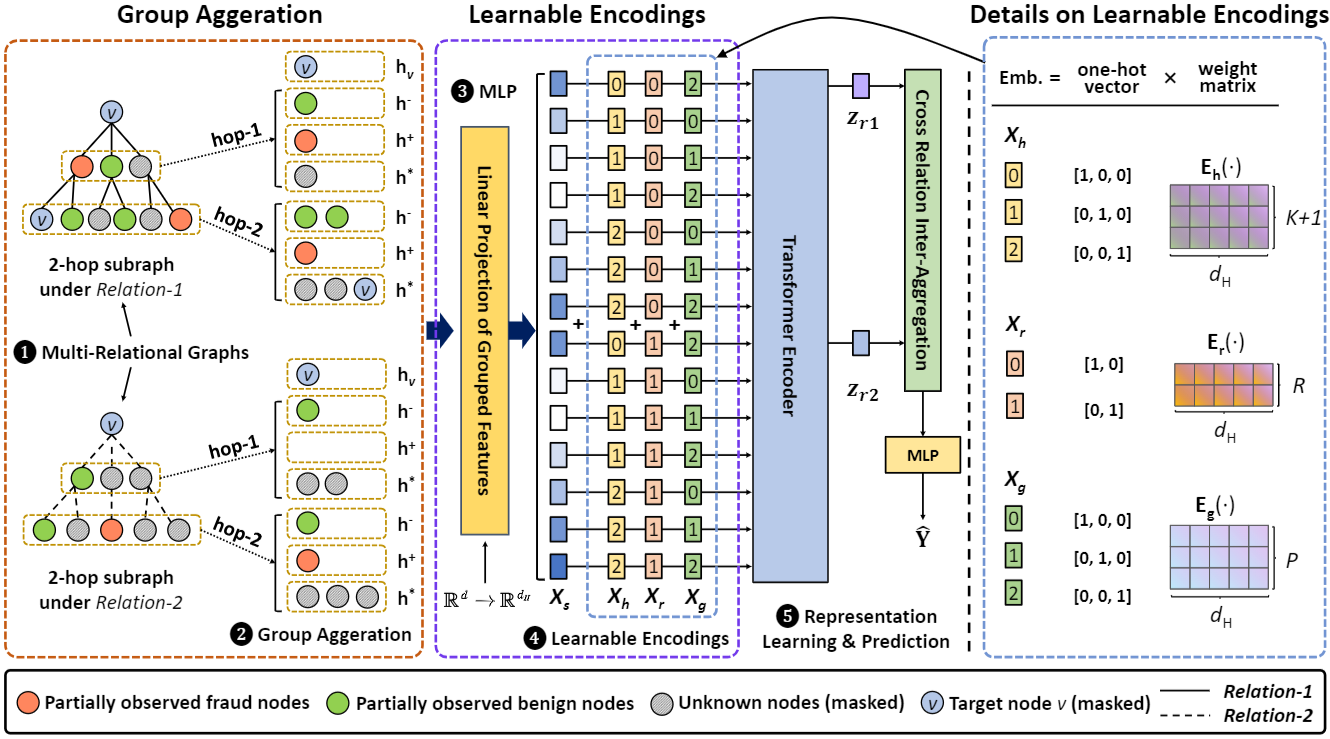
\includegraphics{images/wang2023_arch.png}}
\caption{\label{wang2023_arch} Структура GAGA: под словом hop чаще всего понимают расстояние между двумя вершинами. Соседи узла относятся к hop-1, в свою очередь вершины из их окрестностей, не смежные с данной, будут считаться hop-2 и так далее.}
\end {center}
\end {figure}

Архитектура Dynamic Relation-Attentive Graph (DRAG) \cite{kim2023} использует слой внимания GAT, предварительно добавляя всем узлам петли для нахождения полного самовнимания (self-attention). Исследователи также используют подход формирования метаграфа из NGS, что улучшает производительность модели при меньшем количестве слоев и вычислений. Итоговая архитектура представлена на рис. \ref{kim2023_arch}.

\begin{figure}[ht]
\begin{center}
\scalebox{0.38}{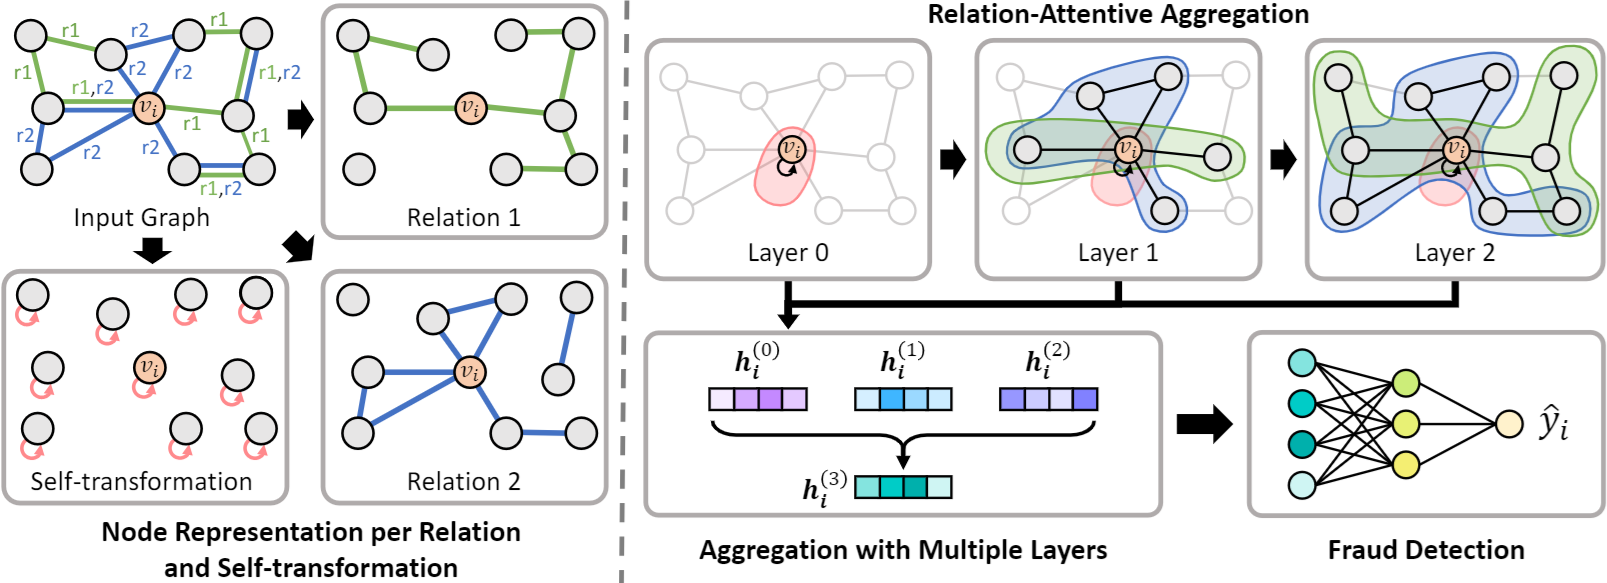
\includegraphics{images/kim2023_arch.png}}
\caption{\label{kim2023_arch} Схема DRAG: разными цветами авторы изобразили несколько типов ребер. Это могут быть связи разного рода, пример такого мультиграфа будет представлен в главе 2.}
\end {center}
\end {figure}

Среди работ, не связанных непосредственно с обнаружением мошенничества на сайтах-агрегаторах отзывов, таких как Amazon и Yelp, можно выделить Exphormer \cite{shirzad2023}, в основе которого лежит другая архитектура General Powerful Scalable graph transformer (GPS) \cite{rampavsek2022}. Авторы применяют слой GAT только к части узлов, сохраняя при этом качество результата. Для этого они строят d-регулярный граф-экспандер на имеющихся вершинах, после используют несколько глобальных узлов, связанных со всеми другими, а затем добавляют полученные ребра к исходному набору. Математически авторы доказывают, что такой подход при использовании нескольких слоев приближается к GAT, но требует меньше операций для вычисления полного самовнимания. При этом полученная работа протестирована на различных задачах, включая классификацию изображений и обнаружение аномальных узлов в графе.

\pagebreak
